%%%%%%%%%%%%%%%%%%%%%%%%%%%%%%%%%%%%%%%%%%%%%%%%%%%%%%%%%%%%%%%%%%%%%%
% How to use writeLaTeX: 
%
% You edit the source code here on the left, and the preview on the
% right shows you the result within a few seconds.
%
% Bookmark this page and share the URL with your co-authors. They can
% edit at the same time!
%
% You can upload figures, bibliographies, custom classes and
% styles using the files menu.
%
%%%%%%%%%%%%%%%%%%%%%%%%%%%%%%%%%%%%%%%%%%%%%%%%%%%%%%%%%%%%%%%%%%%%%%


\documentclass[12pt]{article}

\usepackage{sbc-template}
\usepackage[english]{babel}
\usepackage[utf8]{inputenc}
\usepackage[T1]{fontenc}
\usepackage{graphicx,url}
\usepackage[square,numbers]{natbib}
\usepackage{booktabs}
\usepackage{float}
\usepackage{amsmath}
\usepackage{tikz}
\usepackage{longtable}
\usepackage{enumitem}
\usepackage{placeins}
\usepackage{pdfpages}
\usepackage{textcase}
\usetikzlibrary{arrows.meta, positioning, fit, backgrounds, calc}

% Keeps the file compilable even when a figure has not yet been uploaded to Overleaf.
\newcommand{\safeincludegraphics}[2][]{%
  \IfFileExists{#2}{\includegraphics[#1]{#2}}{%
    \fbox{\parbox{0.86\linewidth}{\centering Missing figure file: \texttt{\detokenize{#2}}}}%
  }%
}

\sloppy

\newcommand{\monografiaAutor}{Rodrigo Neves de Senna Marchiolli}
\newcommand{\monografiaTitulo}{Using Federated Learning to Analyze Occupational Stress: Preserving Privacy and Identifying Patterns}
\newcommand{\monografiaInstituicao}{Universidade Federal de Santa Catarina}
\newcommand{\monografiaCentro}{Centro de Ciências, Tecnologias e Saúde do Campus Araranguá}
\newcommand{\monografiaPrograma}{Curso de Graduação em Engenharia de Computação}
\newcommand{\monografiaTipoTrabalho}{Trabalho de Conclusão de Curso}
\newcommand{\monografiaFormacao}{Bacharel em Engenharia de Computação}
\newcommand{\monografiaLocal}{Araranguá}
\newcommand{\monografiaAno}{2026}
\newcommand{\monografiaCoordenador}{Prof. Antonio Carlos Sobieranski, Dr.}
\newcommand{\monografiaOrientador}{Prof. Martin Vigil, Dr.}
\newcommand{\monografiaAvaliadora}{Profa. Analúcia Schiaffino Morales, Dra.}
\newcommand{\monografiaAvaliador}{Prof. Jim Lau, Dr.}
\newcommand{\monografiaDataAprovacao}{\monografiaAno}
\newcommand{\monografiaOrientadorLinha}{Orientador: \monografiaOrientador}
\newcommand{\monografiaCoorientadorLinha}{}
\newcommand{\monografiaFichaCatalografica}{imagens/ficha_catalografica/Ficha_Catalografica.pdf}

\newcommand{\ufscLogo}{%
  \IfFileExists{setup/vertical_sigla_fundo_claro.pdf}{%
    
\includegraphics[width=1.84cm,keepaspectratio]{setup/vertical_sigla_fundo_claro}\par
  }{%
    \IfFileExists{ref/setup/vertical_sigla_fundo_claro.pdf}{%
      
\includegraphics[width=1.84cm,keepaspectratio]{ref/setup/vertical_sigla_fundo_claro}\par
    }{%
      \textbf{UFSC}\par
    }%
  }%
}

\newcommand{\assinaturaUFSC}[2]{%
  \parbox[t]{0.76\textwidth}{%
    \centering
    \rule{0.68\textwidth}{0.4pt}\\[-1pt]
    #1\\
    #2%
  }%
}

\newcommand{\dataAprovacaoUFSC}{%
  \vspace*{\baselineskip}
  \monografiaLocal, \monografiaDataAprovacao.\par
}

\newcommand{\imprimirfolhaaprovacaoUFSC}{%
  \begin{titlepage}
    \thispagestyle{empty}
    \centering
    \begingroup
    \setlength{\parskip}{0pt}
    \linespread{1.25}\selectfont
    \monografiaAutor\\
    \vspace*{10pt}
    \textbf{\monografiaTitulo}\par
    \vspace*{\baselineskip}
    Este~\monografiaTipoTrabalho~foi julgado adequado para obtenção do Título de~\monografiaFormacao~e aprovado em sua forma final pelo~\monografiaPrograma.\par
    \dataAprovacaoUFSC
    \vspace{22pt}
    \assinaturaUFSC{\monografiaCoordenador}{Coordenador do Curso}\par
    \vspace*{1.4\baselineskip}
    \textbf{Banca Examinadora:}\par
    \vspace{22pt}
    \assinaturaUFSC{\monografiaOrientador}{Orientador}\par
    \vspace{32pt}
    \assinaturaUFSC{\monografiaAvaliadora}{Avaliadora}\par
    \vspace{32pt}
    \assinaturaUFSC{\monografiaAvaliador}{Avaliador}\par
    \endgroup
  \end{titlepage}
}

\newcommand{\imprimircapaUFSC}{%
  \begin{titlepage}
    \thispagestyle{empty}
    \centering
    \begingroup
    \setlength{\parskip}{0pt}
    \linespread{1.25}\selectfont
    \ufscLogo
    \MakeTextUppercase{\monografiaInstituicao}\par
    \MakeTextUppercase{\monografiaCentro}\par
    \MakeTextUppercase{\monografiaPrograma}\par
    \vspace*{5\baselineskip}
    \monografiaAutor\par
    \vspace*{8\baselineskip}
    \textbf{\monografiaTitulo}\par
    \vfill
    \monografiaLocal\par
    \monografiaAno\par
    \endgroup
  \end{titlepage}
}

\newcommand{\imprimirfolhaderostoUFSC}{%
  \begin{titlepage}
    \thispagestyle{empty}
    \centering
    \begingroup
    \setlength{\parskip}{0pt}
    \linespread{1.25}\selectfont
    \vbox to 10cm{%
      \monografiaAutor\par
      \vfill
      \textbf{\monografiaTitulo}\par
    }
    \vfill
    \begin{flushright}
      \begin{minipage}{0.48\textwidth}
        \footnotesize
        \monografiaTipoTrabalho~do~\monografiaPrograma~submetido~ao~\monografiaCentro~da~\monografiaInstituicao~para~a~obtenção~do~título~de~\monografiaFormacao.\par
        \medskip
        \monografiaOrientadorLinha\par
      \end{minipage}
    \end{flushright}
    \vfill
    \monografiaLocal\par
    \monografiaAno
    \endgroup
  \end{titlepage}
}

\newcommand{\imprimirfichacatalograficaUFSC}{%
  \clearpage
  \IfFileExists{\monografiaFichaCatalografica}{%
    \includepdf[pages={1},pagecommand={\thispagestyle{empty}}]{\monografiaFichaCatalografica}
  }{%
    \begin{titlepage}
      \thispagestyle{empty}
      \centering
      \vspace*{\fill}
      Ficha catalográfica não encontrada.
      \vspace*{\fill}
    \end{titlepage}
  }%
}

\newcommand{\imprimirpretextoUFSC}{%
  \imprimircapaUFSC
  \imprimirfolhaderostoUFSC
  \imprimirfichacatalograficaUFSC
  \imprimirfolhaaprovacaoUFSC
  \clearpage
}

\title{\monografiaTitulo}

\author{\monografiaAutor\inst{1}}


\address{Universidade Federal de Santa Catarina (UFSC)\\2026
  \email{rodrigo.nsmarchiolli@gmail.com}
}

\begin{document} 

\imprimirpretextoUFSC

\begin{abstract}
This study evaluated federated learning as a privacy-preserving approach for detecting and monitoring occupational stress. The work combines a literature review with a practical prototype that integrates wearable sensing, a mobile privacy gateway, anonymized communication, authenticated data submission, and local model training. The review discusses the relevance of occupational stress, the role of wearable technologies and artificial intelligence in stress monitoring, and the privacy risks associated with centralized physiological data collection.

For the practical implementation, a layered Internet of Medical Things (IoMT) architecture was developed in which ESP32-based wearable devices transmit physiological signals to an owner-authorized mobile application through authenticated Bluetooth Low Energy bonding. The mobile application stores provisioning credentials securely, signs outgoing JSON payloads with HMAC-SHA256, a Hash-based Message Authentication Code using the SHA-256 hash function, and forwards authenticated requests through the Tor anonymity network to a local training node hosted at a healthcare institution. Local model training was validated on the WESAD dataset using a regularized tabular Multilayer Perceptron (MLP), achieving a validation macro F1-score of 0.9565 for three-class stress classification. The ESP32-based sensing hardware and mobile privacy gateway were functionally validated for data transmission and authentication; the physiological data used for classifier training and validation originated exclusively from the WESAD benchmark dataset, not from the prototype sensors. The proposed model was compared with an original MLP baseline and alternative training strategies, using accuracy, precision, recall \cite{sokolova2009systematic}, macro F1-score, validation loss, and overfitting gap as evaluation criteria. The stress classification component detects general physiological stress states (amusement, baseline, stress) from the WESAD laboratory protocol, not specific occupational stressors; the occupational stress framing is the motivating application context, not the validated experimental scope.
\end{abstract}
    
\begin{resumo}
Este estudo avaliou o aprendizado federado como uma abordagem de preservação de privacidade para detecção e monitoramento de estresse ocupacional. O trabalho combina uma revisão bibliográfica com um protótipo prático que integra sensoriamento vestível, um gateway móvel de privacidade, comunicação anônima, submissão autenticada de dados e treinamento local de modelos. A revisão discute a relevância do estresse ocupacional, o papel das tecnologias vestíveis e da inteligência artificial no monitoramento do estresse e os riscos de privacidade associados à coleta centralizada de dados fisiológicos.

Para a implementação prática, foi desenvolvida uma arquitetura em camadas de Internet das Coisas Médicas (IoMT) na qual dispositivos vestíveis baseados em ESP32 transmitem sinais fisiológicos para um aplicativo móvel autorizado pelo proprietário por meio de emparelhamento autenticado Bluetooth Low Energy. O aplicativo móvel armazena credenciais de provisionamento de forma segura, assina payloads JSON de saída com HMAC-SHA256, um Código de Autenticação de Mensagem baseado em Hash usando a função hash SHA-256, e encaminha requisições autenticadas através da rede de anonimato Tor para um nó de treinamento local hospedado em uma instituição de saúde. O treinamento local do modelo foi validado no conjunto de dados WESAD usando um Perceptron Multicamadas (MLP) tabular regularizado, alcançando um macro F1-score de validação de 0,9565 para classificação de estresse em três classes. O hardware de sensoriamento baseado em ESP32 e o gateway móvel de privacidade foram funcionalmente validados para transmissão de dados e autenticação; os dados fisiológicos usados para treinamento e validação do classificador foram originados exclusivamente do conjunto de dados de referência WESAD, e não dos sensores do protótipo. O modelo proposto foi comparado com uma MLP baseline original e estratégias alternativas de treinamento, utilizando acurácia, precisão, recall, macro F1-score, perda de validação e gap de overfitting como critérios de avaliação. O componente de classificação de estresse detecta estados fisiológicos gerais de estresse (amusement, baseline, stress) do protocolo laboratorial WESAD, e não estressores ocupacionais específicos; o contexto de estresse ocupacional é a motivação aplicada, não o escopo experimental validado.
\end{resumo}

\section{Introduction}


Occupational stress, a significant concern in contemporary work environments, stems from the imbalance between job-related pressures and an individual's ability to cope with them, precipitating a range of detrimental consequences for personal health and organizational effectiveness. Given that occupational stress is not a condition that can be cured through treatment but rather a risk factor requiring consideration of the problem's history, continuous monitoring and proactive management become paramount \cite{james_campbell_quick_f0fffc85}. The repercussions of occupational stress are multifaceted, impacting individual well-being through emotional distress and physical health problems, while also affecting organizations via diminished productivity and increased costs \cite{james_campbell_quick_f0fffc85, paul_e__spector_2bae7a3d, shiyi_jiang_d0702d3b}. The current work environment's demands often clash with employees' physiological, emotional, and social needs, making it essential to create supportive work conditions that encourage growth and productivity while aiding individuals in their challenges \cite{agnese_mariotti_dd5ad5ca}. 


Wearable technology and artificial intelligence offer innovative pathways for detecting and managing occupational stress by continuously monitoring physiological signals and behaviors linked to stress responses \cite{james_campbell_quick_f0fffc85}. The integration of wearable sensors, coupled with advanced data analytics, creates opportunities for real-time insights into an individual's stress levels, thereby enabling the implementation of timely and personalized intervention strategies \cite{reham_alhejaili_14968434, mazin_alshamrani_65eed49a}. Such interventions have the potential to mitigate the adverse effects of stress, fostering healthier and more productive work environments \cite{jerry_chen_fd58cab0}. However, the traditional centralized data collection approach raises significant concerns regarding privacy and data security. The centralized storage and processing of sensitive employee data, such as physiological information and behavioral patterns, can expose individuals to potential breaches, unauthorized access, and misuse of their personal information. This poses substantial risks to both employee privacy and organizational data security. To address these concerns, alternative approaches that prioritize privacy and security while still enabling effective occupational stress analysis are needed.

Federated learning, a decentralized machine learning technique, addresses these privacy issues by allowing models to be trained locally on individual devices without sharing sensitive raw data \cite{yekta_said_can_3e1184b6, ziyu_wang_a7666f66}. This approach holds significant promise for occupational stress analysis, as it enables the preservation of employee privacy and data security. In contrast to traditional centralized machine learning methods, which involve the collection and storage of raw physiological and behavioral data, federated learning empowers individuals to train models on their own devices, sharing only model updates rather than the underlying personal information \cite{muhammad_ali_fauzi_c546a580}.

By leveraging federated learning, this study aims to explore its potential for analyzing occupational stress, emphasizing the dual objectives of accurate stress detection and the protection of data privacy. The practical prototype extends this vision with a mobile privacy gateway that routes authenticated physiological data through the Tor network to local training nodes at healthcare institutions, ensuring that raw signals remain on-premises while only model updates participate in global aggregation. After aggregation via Federated Averaging (FedAvg), the global server redistributes the updated aggregated weights back to the participating clients, enabling collaborative model improvement without exposing raw data.

Through a literature review and practical implementation, this research intends to assess the effectiveness and advantages of federated learning compared to traditional centralized methods. By combining local model training with a privacy-preserving communication path based on Tor and HMAC-SHA256 (Hash-based Message Authentication Code using the SHA-256 hash function), this work seeks not only to enhance privacy and data security, but also to maintain the precision and accuracy of stress detection models in realistic occupational health scenarios. In this context, Tor hides the network origin of the request, while HMAC-SHA256 verifies message integrity and authorization at the application layer. Additionally, the research aims to demonstrate the practical applicability and benefits of federated learning in addressing occupational stress, a critical issue with significant social, economic, and organizational implications. It is important to distinguish two validation dimensions: the end-to-end hardware and software architecture (ESP32, BLE, Tor, HMAC, Flower) was implemented and functionally tested; the stress classification model, however, was trained and validated using the public WESAD dataset, not data collected by the prototype sensors in a live deployment.

The scope of the term "occupational stress" as used in this work also requires clarification. Occupational stress is a multifactorial phenomenon involving environmental, emotional, organizational, and psychosocial stressors that vary across work contexts \cite{morales2026affective}. The present study, however, validates a classifier for general physiological stress states (amusement, baseline, stress) induced under controlled laboratory conditions following the WESAD protocol. The occupational health motivation justifies the investigation, but the experimental validation does not fully replicate the real-world spectrum of occupational stressors. This distinction should be considered when interpreting the results.

This paper is organized into seven sections. Section 2 details the methodology employed in the literature review, investigating four databases: PubMed, IEEE Xplore, Scopus, and Web of Science; based on inclusion and exclusion criteria, a total of 11 scientific articles were selected. Section 3 presents the main results of the literature review, addressing the research questions and related discussions. Section 4 covers the main challenges encountered and solutions implemented during the development of the privacy-preserving prototype. Section 5 presents the practical results, Section 6 discusses the implications of these findings, and Section 7 concludes the study.

\section{Methodology}

This research employed a mixed-methods approach, incorporating a literature review and practical implementation to evaluate the effectiveness and security of federated learning for detecting and monitoring occupational stress. 

The literature review followed PRISMA guidelines, ensuring a structured process for identifying, selecting, and synthesizing relevant studies. The literature review aimed to explore the current state of research on federated learning, traditional machine learning, occupational stress, and wearable technologies, providing a comprehensive understanding of the field. 

The review process consisted of well-defined steps: (1) formulating research questions; (2) identifying relevant literature; (3) applying selection criteria to filter articles; (4) extracting and analyzing data; and (5) synthesizing and presenting the findings.


\subsection{Formulating Research Questions}

To guide the literature review, the following research questions were established:
\begin{itemize}
    \item \textbf{RQ1}: How can data security and privacy be ensured in the context of federated learning?
    \item \textbf{RQ2}: What types of machine learning algorithms are commonly employed in federated learning for occupational stress analysis?
    \item \textbf{RQ3}: What are the primary challenges and limitations of federated learning in real-world occupational settings?
    \item \textbf{RQ4}: How can federated learning be integrated with wearable technology for continuous and personalized occupational stress monitoring?
    \item \textbf{RQ5}: What are the main challenges and corresponding solutions found in applying federated learning for occupational stress monitoring?
\end{itemize}

\subsection{Identifying Relevant Literature}


Four academic databases were systematically searched: PubMed, IEEE Xplore, Scopus, and Web of Science, chosen for their extensive collections of peer-reviewed literature in health sciences, technology, and engineering. 

Articles were selected based on well-defined inclusion criteria as described in Table~\ref{tab:criterios}, such as peer-reviewed status, publication date (recent ten years), focus on federated learning, stress monitoring, and wearable technology. Articles that did not meet these criteria or lacked sufficient methodological detail were excluded. The selection process involved title and abstract screening, followed by full-text evaluation.

\begin{table}[htbp]
\centering
\caption{Inclusion and Exclusion Criteria}
\label{tab:criterios}
\resizebox{\textwidth}{!}{%
\begin{tabular}{p{7cm} p{7cm}}
\toprule
\textbf{Inclusion Criteria} & \textbf{Exclusion Criteria} \\ \midrule
Studies on Federated Learning and stress & Duplicate articles \\ \midrule
Contribution to research questions & Articles not available in full text \\ \midrule
Available in full version & Studies outside the scope \\ \midrule
Peer-reviewed status & Review articles \\ \bottomrule
\end{tabular}%
}
\end{table}

\subsection{Applying Selection Criteria to Filter Articles}

The search was conducted in Web of Science, Scopus, PubMed, and IEEE Xplore databases using the following search string to ensure relevance: ("occupational stress" OR "workplace stress" OR stress) AND "federated learning". The specific search strings and adjustments for each database were as follows:

\begin{itemize}
    \item \textbf{Web of Science}
    \begin{itemize}
        \item Search String: \texttt{ALL=(("occupational stress" OR "workplace stress" OR stress) AND "federated learning")}
        \item Adjustments: Display final publication year
        \item Initial number of articles: 34
    \end{itemize}
    \item \textbf{Scopus}
    \begin{itemize}
        \item Search String: \texttt{TITLE-ABS-KEY ( ( "occupational stress" OR "workplace stress" OR stress ) AND "federated learning" )}
        \item Adjustments: Include only the document type \textit{Article}
        \item Initial number of articles: 10
    \end{itemize}
    \item \textbf{PubMed}
    \begin{itemize}
        \item Search String: \texttt{("occupational stress"[Title/Abstract] OR "workplace stress"[Title/Abstract] OR stress[Title/Abstract]) AND "federated learning"[Title/Abstract]}
        \item Initial number of articles: 5
    \end{itemize}
    \item \textbf{IEEE Xplore}
    \begin{itemize}
        \item Search String: \texttt{("All Metadata":federated learning) AND ("All Metadata":occupational stress OR "All Metadata":workplace stress OR "All Metadata":stress)}
        \item Initial number of articles: 41
    \end{itemize}
\end{itemize}

The review process began with 90 articles from the Web of Science, Scopus, PubMed, and IEEE Xplore databases. The RAYYAN tool was used to assist in the selection \cite{nastasha_johnson_93d644ed}. After removing 29 duplicates, 61 articles were screened. Of these, 34 were excluded based on the title and abstract. The remaining 27 were retrieved in full and assessed using the inclusion and exclusion criteria. Sixteen articles were excluded for not meeting the criteria or being out of scope. Ultimately, 11 articles were included in the literature review. The PRISMA flow diagram in Figure~\ref{fig:prisma} details this selection process. Table~\ref{tab:included_articles} summarizes these 11 articles, their focus, algorithms, datasets, and relationship to the implemented prototype.

\begin{figure}[htbp]
    \centering
    \safeincludegraphics[width=0.8\linewidth]{imagens/prisma.png}
    \caption{PRISMA flow diagram}
    \label{fig:prisma}
\end{figure}

\begingroup
\small
\setlength{\tabcolsep}{4pt}
\renewcommand{\arraystretch}{1.08}

\begin{longtable}{p{4.5cm} p{3.2cm} p{2.2cm} p{2.8cm} p{1.4cm}}
\caption{Summary of articles included in the literature review.}
\label{tab:included_articles} \\

\toprule
\textbf{Reference} & \textbf{Focus} & \textbf{ML/FL Algorithm} & \textbf{Physiological Data/Dataset} & \textbf{Relationship} \\ \midrule
\endfirsthead

\caption[]{Summary of articles included in the literature review. (Continued)} \\

\toprule
\textbf{Reference} & \textbf{Focus} & \textbf{ML/FL Algorithm} & \textbf{Physiological Data/Dataset} & \textbf{Relationship} \\ \midrule
\endhead

\bottomrule
\endfoot

\cite{abdulrahman_alahmadi_32bc288c} & Privacy-preserved IoMT stress detection & FL, ANN, RF, k-NN & WESAD (ECG, EDA, EMG, Resp, TEMP) & Direta \\ \midrule

\cite{ahmad_almadhor_8cc2e670} & FL-based stress detection with edge computing & FL, DNN & WESAD (EDA) & Direta \\ \midrule

\cite{yekta_said_can_3e1184b6} & Privacy-preserving FL for wearable IoT & FL, Deep Learning & Heart activity (smart bands) & Direta \\ \midrule

\cite{neha_gahlan_d8b04f5d} & FL inspired privacy sensitive emotion recognition & FL, CNN & Multi-modal physiological sensors & Parcial \\ \midrule

\cite{jayant_vyas_bcd9860b} & Driver recommendation using FL & FL, Multi-task Learning & UAH-DriveSet, HCI Lab, PhysioNet & Parcial \\ \midrule

\cite{m__bharathi_b0a198b0} & FL for healthcare IoT: origins and applications & FL, ML & Healthcare IoT & Parcial \\ \midrule

\cite{mohamed_benouis_35501772} & FL for mental health monitoring & FL, Multi-task Learning & Multimodal physiological signals & Parcial \\ \midrule

\cite{jessica_chia_liu_cd0e0973} & FL for health data privacy & FL (simulation) & Wearable physiological and motion data & Contextual \\ \midrule

\cite{nastasha_johnson_93d644ed} & RAYYAN systematic review tool & N/A & N/A & Contextual \\ \midrule

\cite{adam_sadilek_c59c73f4} & Privacy-first health research with FL & FL, Differential Privacy & Multi-site health studies & Contextual \\ \midrule

\cite{chuan_ma_e07241ba} & Data privacy and security in FL & FL, privacy techniques & Simulated data & Contextual \\

\end{longtable}

\endgroup



\section{Main Results and Discussion}

\subsection{\textit{RQ1}: How can data security and privacy be ensured in the context of federated learning?}


Federated learning (FL) provides inherent advantages for preserving data privacy by ensuring that sensitive information remains decentralized, a crucial requirement when dealing with confidential healthcare datasets \cite{adam_sadilek_c59c73f4} [Contextual]. This approach minimizes the risks associated with data breaches and unauthorized access, aligning with stringent data protection regulations such as the General Data Protection Regulation (GDPR) and HIPAA \cite{m__bharathi_b0a198b0} [Parcial]. Several strategies enhance data security and privacy within federated learning frameworks, including differential privacy, homomorphic encryption, and secure multi-party computation \cite{jie_xu_193cbfb6}. Blockchain-orchestrated FL architectures have also been proposed for healthcare consortia, combining distributed ledger immutability with decentralized model training to strengthen data governance across participating institutions \cite{jonathan_passerat_palmbach_a7961671}.

In addition, regulations such as GDPR reinforce the importance of privacy-preserving technologies, highlighting the crucial role of FL in complying with specific data protection legislation. In this context, complementary techniques have been explored to strengthen security and privacy in FL, including physical transmission layer security mechanisms, such as leveraging the unique properties of wireless channels to protect communications between local devices and central servers. By focusing on safeguarding both the client and server sides, federated learning addresses critical aspects such as convergence, data poisoning, scaling, and model aggregation \cite{chuan_ma_e07241ba} [Contextual]. In addition, FL has been applied to network intrusion detection in smart environments, further demonstrating its versatility in securing distributed healthcare and IoT systems \cite{cholakoska2023federated}.

Other advanced techniques have also been incorporated into FL to increase the protection of shared data. For example, the use of Generative Adversarial Networks (GANs) for data augmentation and Graph Attention Networks (GATs) have been explored in the literature to improve learning from distributed data while limiting the amount of information exchanged, further reducing the possibility of inferring sensitive information through reverse engineering. \cite{shiyi_jiang_49d728e9}.

Therefore, FL ensures data security and privacy mainly by keeping raw information locally, sharing exclusively the parameters of trained models and incorporating additional techniques such as Differential Privacy, advanced encryption and specific machine learning methods, which together provide robust protection against privacy attacks without compromising the performance of the developed systems.
    
\subsection{\textit{RQ2}: What types of machine learning algorithms are commonly employed in federated learning for occupational stress analysis?}

There is no universal approach when developing artificial intelligence models applied to federated learning (FL) for occupational stress analysis. Specialized literature suggests various algorithms commonly used due to their proven capability to handle specific federated learning challenges, such as data decentralization, information privacy, and device heterogeneity \cite{adam_sadilek_c59c73f4} [Contextual].

Among the most employed algorithms are \textit{Artificial Neural Networks (ANN)}, \textit{Random Forest (RF)}, \textit{Support Vector Machines (SVM)}, \textit{k-Nearest Neighbors (k-NN)}, and \textit{Logistic Regression (LR)}. Each of these techniques has distinct characteristics and advantages suitable for practical applications in federated environments for occupational stress analysis.

A visual comparison summarizing the main algorithms discussed can be observed in Table~\ref{tab:algorithms_comparison}.

To provide context for the performance expectations of these algorithms, a recent meta-analysis of wearable-based stress detection studies reported a pooled mean accuracy of 85.6\% (95\% CI 70--93\%) across 71 accuracy estimates from 17 studies, with individual algorithm performances varying according to dataset, validation protocol, and classification granularity \cite{alaa_abd-alrazaq_e52622}.

\subsubsection{Artificial Neural Networks (ANN)}

Artificial Neural Networks are highly versatile algorithms inspired by the human brain's structure, capable of modeling complex relationships between input data (e.g., physiological signals acquired by wearable sensors) and outputs (e.g., detected stress levels). ANNs are particularly valued for their ability to extract non-linear patterns from multidimensional and heterogeneous data \cite{abdulrahman_alahmadi_32bc288c} [Direta]. In federated learning contexts, they are widely adopted due to their flexibility in handling diverse physiological data types, such as electrocardiogram (ECG), electrodermal activity (EDA), and electromyography (EMG), along with effective adaptation to edge devices with computational resource constraints \cite{abdulrahman_alahmadi_32bc288c}.

\textbf{Challenges:} Requires large data volume and high local computational resources.

\subsubsection{Random Forest (RF)}

Random Forest is an ensemble method algorithm that combines results from multiple individual decision trees. The main strength of this method lies in its robustness against noisy data and its capacity to avoid overfitting, which is critically advantageous in federated learning environments where data quality can vary significantly among participants. In this context, protecting the aggregation from anomalies or malicious updates is crucial to maintain robustness, being investigated through mechanisms like latent space inspection and autoencoders to secure threat detection models \cite{tran_duc_luong_b5df10e8}. Additionally, RF is particularly effective for physiological data, allowing accurate classification by consolidating multiple decisions from distributed devices, thereby reducing reliance on a single model or data source \cite{adam_sadilek_c59c73f4}.

\textbf{Challenges:} Potentially higher complexity when employing numerous trees on resource-limited devices.

\subsubsection{Support Vector Machines (SVM)}

SVM is widely recognized for effectively classifying complex data by establishing clear separation hyperplanes between classes. This method consistently performs well in FL contexts for detecting physiological states related to stress, particularly when client-specific data availability is limited. Nonetheless, SVM requires careful parameter tuning to handle non-linear and noisy data, frequently encountered in stress analysis from wearable sensors. To evaluate such challenges in practical environments, researchers propose physical testbeds with frameworks like Flower and embedded hardware to analyze model resilience under adverse conditions \cite{hao_huang_8976046f}.

\textbf{Challenges:} Complex hyperparameter tuning and sensitivity to outliers.

\subsubsection{k-Nearest Neighbors (k-NN)}

The k-NN algorithm is a simple yet effective method that classifies new data points based on the labels of their \textit{k} nearest neighbors. In federated learning, its simplicity and low computational cost are particularly valuable, facilitating direct implementation on wearable devices with limited resources. However, challenges such as noisy data, local distribution heterogeneity, and class imbalance must be managed carefully to ensure reliable results. Advanced techniques, such as SMOTE or SMOTEENN, can mitigate imbalance issues that could compromise accuracy \cite{abdulrahman_alahmadi_32bc288c}.

\textbf{Challenges:} High computational cost during prediction with large datasets.

\subsubsection{Logistic Regression (LR)}

Logistic Regression is a classic method for binary classification problems, modeling the probability that a data point belongs to a class based on explanatory variables. In FL, its primary advantage is simplicity, fast training, and low computational requirement, aspects that facilitate deployment on distributed devices. Nevertheless, it is sensitive to data balance and representativeness, demanding careful parameter tuning and additional strategies to prevent overfitting. Its applicability in federated environments is mainly explored when straightforward interpretation of variables is required \cite{abdulrahman_alahmadi_32bc288c}.

\textbf{Challenges:} Sensitive to data imbalance.

\subsubsection{Other Relevant Algorithms}

Beyond the mentioned techniques, there is growing interest in using more complex algorithms, such as Convolutional Neural Networks (CNN) and Recurrent Neural Networks (RNN), specifically designed for analyzing sequential and temporal data acquired by wearable sensors \cite{yekta_said_can_3e1184b6} [Direta]. Hybrid techniques and Multi-task Learning (MTL) methods have also been proposed to enhance federated model accuracy and robustness by sharing representations across related tasks\cite{mohamed_benouis_35501772} [Parcial].

Ensemble learning techniques, like Gradient Boosting Machines and AdaBoost, are also highlighted for significantly improving predictive performance by combining multiple individual models, thus enhancing generalization capability in heterogeneous federated data scenarios \cite{alaa_abd-alrazaq_e52622}.

\begin{table}[htbp]
\centering
\caption{Visual comparison of commonly employed machine learning algorithms in federated learning for occupational stress analysis.}
\label{tab:algorithms_comparison}
\resizebox{\textwidth}{!}{%
\begin{tabular}{lccccccl}
\toprule
\textbf{Algorithm} & \textbf{Type} & \textbf{Reported Performance} & \textbf{Noise Robustness} & \textbf{Computational Cost} & \textbf{Suitability for FL} & \textbf{Reference} \\ \midrule
ANN                & Non-linear    & Varies             & Medium                    & High                        & High                        & \cite{alaa_abd-alrazaq_e52622} \\ \midrule
Random Forest      & Non-linear    & Varies             & High                      & Medium-High                 & High                        & \cite{adam_sadilek_c59c73f4} \\ \midrule
SVM                & Linear/Non-linear & Varies            & Medium                    & Medium-High                 & Medium                      & \cite{hao_huang_8976046f} \\ \midrule
k-NN               & Non-linear    & Varies             & Low                       & Medium-Low                  & Medium                      & \cite{alaa_abd-alrazaq_e52622} \\ \midrule
Logistic Regression & Linear       & Varies             & Low-Medium                & Low                         & High                        & \cite{alaa_abd-alrazaq_e52622} \\ 
\bottomrule
\end{tabular}%
}
\end{table}

These descriptions and visual comparisons provide a comprehensive foundation, clearly illustrating each algorithm's technical characteristics and practical applicability in federated learning contexts for occupational stress detection.

\subsection{\textit{RQ3}: What are the primary challenges and limitations of federated learning in real-world occupational settings?}


Federated learning, while promising, faces significant challenges in real-world occupational settings, primarily due to issues related to data heterogeneity, communication constraints, and system scalability \cite{shiyi_jiang_49d728e9}. Data heterogeneity arises from variations in sensor types, data collection protocols, and individual physiological responses, making it difficult to train a globally consistent model \cite{po_chen_lin_822ae077}. 

Communication constraints, particularly in scenarios with limited bandwidth or intermittent connectivity, pose challenges for model aggregation and distribution \cite{tian_li_4bd16a66}. Addressing statistical heterogeneity, also known as non-IID (independent and identically distributed) data, is paramount in federated learning because the distribution of local data across different clients can vary significantly due to diverse occupational environments and individual differences, which impacts model convergence and performance. 

Furthermore, the computational capabilities of edge devices used for local training can vary widely, creating additional challenges for deploying complex models and algorithms \cite{neha_gahlan_d8b04f5d} [Parcial].  Moreover, security and privacy considerations are paramount, necessitating robust mechanisms to defend against adversarial attacks such as data poisoning and inference attacks, while simultaneously ensuring adherence to stringent data protection regulations such as GDPR and HIPAA, which mandate the safeguarding of sensitive health information \cite{bouacida2021vulnerabilities,adam_sadilek_c59c73f4} [Contextual].

The trustworthiness of federated learning systems is also a major concern, requiring careful attention to issues such as data quality, provenance, and bias detection to ensure reliable and equitable outcomes \cite{jie_xu_193cbfb6}.

The lack of standardized benchmarks and evaluation metrics makes it difficult to compare the performance of different federated learning approaches and assess their suitability for specific occupational settings. 

Therefore, addressing these challenges requires interdisciplinary collaboration involving experts in machine learning, cybersecurity, and occupational health, along with the development of innovative solutions that balance privacy, accuracy, and efficiency.


\subsection{\textit{RQ4}: How can federated learning be integrated with wearable technology for continuous and personalized occupational stress monitoring?}

Federated learning can be seamlessly integrated with wearable technology to enable continuous and personalized occupational stress monitoring, offering numerous advantages over traditional centralized approaches. By processing data locally on wearable devices, federated learning minimizes the need to transmit sensitive physiological data to a central server, thereby reducing the risk of data breaches and privacy violations \cite{jessica_chia_liu_cd0e0973} [Contextual]. Wearable devices, equipped with sensors such as heart rate monitors and electrodermal activity sensors, continuously collect physiological data, which is then pre-processed and analyzed locally using lightweight machine learning models. 

FL operates by training models locally on individual wearable devices or edge devices such as smartphones. Each device can collect physiological signals such as BVP/PPG, EDA, respiration, skin temperature, ECG, or EMG, depending on the wearable configuration; these signals are commonly explored as indicators of stress-related physiological responses \cite{abdulrahman_alahmadi_32bc288c} [Direta]. 

These models are trained using algorithms such as federated averaging, which aggregates model updates from multiple devices to create a global model without directly accessing the raw data.  

Additionally, the effectiveness of these technologies depends on their ability to accurately capture and interpret physiological signals indicative of stress \cite{ahmad_almadhor_8cc2e670} [Direta].

Federated learning further preserves data privacy and promotes real-time distribution of models and learning by enabling devices to collaboratively train and evaluate a shared model while keeping personal data on site. Moreover, federated learning enables personalized stress models that adapt to individual physiological characteristics and work patterns, leading to more accurate and timely stress detection. The integration of federated learning with wearable technology requires careful consideration of factors such as device heterogeneity, communication bandwidth, and energy efficiency to ensure optimal performance and user experience.

\subsection{\textit{RQ5}: What are the main challenges and the corresponding solutions found in applying federated learning for occupational stress monitoring?}


Applying federated learning to occupational stress monitoring presents several challenges related to data quality, privacy, and computational resources, which necessitate innovative solutions to ensure effective and reliable monitoring \cite{ahmad_almadhor_8cc2e670} [Direta], \cite{abdulrahman_alahmadi_32bc288c} [Direta]. Data quality can be affected by sensor noise, missing values, and individual variations in physiological responses, which can impact the accuracy of stress detection models. 

To address these challenges, robust data preprocessing techniques such as filtering, imputation, and normalization are essential to improve the quality and consistency of the data used for training federated learning models. Differential privacy mechanisms, such as adding noise to model updates, can be employed to protect sensitive data from inference attacks, but this must be done carefully to avoid compromising model accuracy. 

One of the primary advantages of federated learning is its ability to maintain data privacy by processing data locally on user devices \cite{jakub_kone_n__e9c179d4}. This decentralized paradigm has also been successfully adapted to other smart home monitoring scenarios, such as non-intrusive load monitoring (NILM) for smart grid applications, showcasing its versatility in preserving privacy at the edge \cite{shuang_dai_ae9ca8bc}. 

The inherent architecture of federated learning prioritizes user privacy, as model training occurs on decentralized devices, and only model updates are shared with a central server \cite{tomer_gafni_ff1f0d6e}. 

The heterogeneity of wearable devices and communication networks in occupational settings poses another challenge, requiring adaptive learning algorithms and communication protocols that can accommodate variations in computational resources and network bandwidth \cite{po_chen_lin_822ae077}.   

Despite these challenges, federated learning has been found to hold great promise in improving the detection and management of occupational stress. 

\section{Challenges Encountered and Solutions Implemented}

During the practical phase of this research, the original architecture, in which ESP32 devices would communicate directly with a local MQTT gateway and then traverse the Tor network, was refined. The final prototype delegates network-intensive operations to a mobile application, which acts as an intermediary between wearable sensors and the local training node hosted at a healthcare institution. This decision reflects hardware constraints on embedded devices, which cannot efficiently run a full Tor client for continuous operation, while preserving the privacy goals outlined in the literature review.

\subsection{Embedded Device and Network Constraints}

A first challenge was the limited computational capacity of ESP32-based wearable devices. The ESP32 is a low-cost microcontroller commonly used in Internet of Things prototypes; it is appropriate for reading sensors and sending compact messages, but not for maintaining a full anonymized communication stack continuously. The implemented solution was to keep the wearable layer focused on sensing and to move Tor connectivity, QR provisioning, secure storage, and request signing to the smartphone. In this work, Tor is used as an anonymity network that hides the network origin of the request, QR provisioning is the process of configuring the application through a QR code, and request signing is the process of attaching a cryptographic proof that the message was produced by an authorized client. This preserves the feasibility of the Internet of Medical Things (IoMT) layer while maintaining network-level privacy through the mobile gateway.

\subsection{Credential Provisioning and Request Authentication}

A second challenge was how to authorize incoming requests without exposing secrets in transit. The solution was a QR-based provisioning workflow. The local API generates credentials containing the hidden service address and a shared password. A hidden service address is a Tor address ending in \texttt{.onion}, which allows the hospital-side service to be reached through the Tor network without exposing a conventional public IP address. The mobile application scans this QR code, stores the credentials locally, serializes the outgoing JSON body, and computes an HMAC-SHA256 (Hash-based Message Authentication Code using the SHA-256 hash function) signature over the exact payload bytes. HMAC-SHA256 is a keyed hash: it uses a shared secret and the message content to produce a signature that can be verified by the server, without sending the secret itself. The server recomputes the signature and rejects requests with invalid signatures. This mechanism adds integrity and authorization to the anonymous communication channel provided by Tor.

\subsection{Local Model Design for WESAD Validation}

A third challenge was choosing a model compatible with the actual feature representation used in this work. The WESAD preprocessing pipeline converts physiological signals into 30-second windows represented as tabular feature vectors, meaning that each observation is a row of numerical measurements rather than a raw time series. Therefore, the practical validation used a tabular Multilayer Perceptron (MLP), a neural network composed of fully connected layers, rather than a temporal model such as an LSTM, GRU, 1D-CNN, or transformer. The improved model includes regularization and training-stability mechanisms such as normalization inside the network, dropout, class-weighted loss, learning-rate scheduling, early stopping, gradient clipping, and light Gaussian noise augmentation. These mechanisms are described in more detail in Section~5, where they are connected to the experimental results.

\subsection{WESAD Dataset Characterization}

The Wearable Stress and Affect Detection (WESAD) dataset \cite{philip_schmidt_382e77a1} is a publicly available multimodal corpus for stress and affect recognition from wearable physiological sensors. It was collected by Schmidt et al. (2018) at the University of Trier, Germany, following a controlled laboratory protocol based on the Trier Social Stress Test (TSST) with an added positive affective induction. Fifteen participants (n = 15) were exposed to three experimental conditions: baseline (neutral relaxation), amusement (watching humorous video clips), and stress (public speaking and mental arithmetic). Physiological signals were recorded from two wearable placements: a chest-worn RespiBAN device capturing electrocardiogram (ECG), electromyography (EMG), electrodermal activity (EDA), respiration (Resp), and skin temperature (TEMP); and a wrist-worn Empatica E4 device capturing blood volume pulse (BVP), electrodermal activity (EDA), and skin temperature (TEMP). The resulting dataset contains approximately 36 minutes of labeled multi-modal physiological recordings per participant. WESAD was chosen for validation because it provides a controlled benchmark with signal modalities compatible with the proposed wearable prototype and allows reproducible comparisons with prior federated learning and stress classification studies \cite{abdulrahman_alahmadi_32bc288c, ahmad_almadhor_8cc2e670, neha_gahlan_d8b04f5d}.

\subsection{Privacy-Oriented Feature Selection}

The use of demographic attributes such as age, height, and weight created a privacy concern because these variables may act as quasi-identifiers. To evaluate this issue, a second version of the training script removed these features and retained only the physiological feature set. This demographics-free configuration produced a modest reduction in validation macro F1-score while preserving competitive performance, supporting the feasibility of a more privacy-conscious deployment.

\subsection{Federated Learning Integration Scope}

The current prototype validates the data ingestion, authentication, anonymized transport, local WESAD training, and software integration path for Flower-based federated learning. Flower is the framework used to coordinate federated training rounds. At the beginning of each round, the global Flower server sends the current global model parameters to a subset of available Flower clients. Each client, three simulated institutional nodes in this prototype, receives these parameters, initializes its local TabularMLP with them, and trains on its own partition of the WESAD dataset. The 805 training windows are split into three non-overlapping subsets of approximately 268 windows each. After local training, each client sends its updated model parameters back to the global server, which aggregates them using Federated Averaging (FedAvg). The FedAvg algorithm computes a weighted mean of the client parameter updates, producing a new global model. This model is then redistributed to the clients for the next round. The simulation runs for 15 to 20 federated rounds, after which the global model converges. The results reported in this paper should therefore be interpreted as validation of the local client-side training pipeline and of the surrounding privacy-preserving communication architecture. They should not yet be interpreted as a completed multi-institutional benchmark with independent real hospital datasets.

\section{Results}

This section presents the practical outcomes of the project, organized according to the evolved system architecture. The implementation combines wearable physiological sensing, a mobile privacy gateway, network anonymization through Tor, application-layer authentication via HMAC, local data storage at the institutional node, federated training with Flower, and model redistribution to the mobile application. The WESAD dataset is used as a validation benchmark for the stress classification pipeline.

To make the results self-contained, the glossary in Appendix~A (Table~\ref{tab:technical_terms_results}) summarizes the main technical terms used throughout this section and their role in the implemented prototype.



\subsection{Mobile Application as Privacy Gateway}

The mobile application was developed as an Expo/React Native prototype with native modules for Tor connectivity, camera-based QR code scanning, secure credential storage, and communication with the ESP32-based sensing unit. Expo/React Native was used because it supports mobile interface development in JavaScript/TypeScript while still allowing native modules for capabilities such as Bluetooth and Tor connectivity. This design addresses a central limitation identified during prototyping: executing a Tor daemon directly on ESP32 hardware is computationally prohibitive for continuous operation. By contrast, modern smartphones provide sufficient resources to run a native Tor client while maintaining an intuitive interface for credential provisioning, local request preparation, and secure data submission.

In the proposed workflow, a single ESP32 simulates the collection of pre-recorded physiological signals from the WESAD dataset, reading them from FLASH memory and transmitting them via BLE to the mobile gateway. Wrist or pulse sensors provide BVP, EDA, and skin temperature measurements. BVP, or blood volume pulse, captures changes in blood flow and is related to cardiovascular response. EDA, or electrodermal activity, captures changes in skin conductance and is commonly associated with sympathetic nervous system activation. The chest sensor provides respiratory data through a strain gauge, which detects expansion and contraction during breathing. The ESP32 transmits these physiological readings to the mobile application through authenticated Bluetooth Low Energy bonding. The smartphone then acts as a privacy gateway between the local sensing layer and the hospital-side training infrastructure.

The mobile gateway pipeline comprises three main stages:

\begin{enumerate}[leftmargin=*]
\item \textbf{Credential provisioning:} the local training node API generates a QR code containing a JSON object with the \texttt{.onion} service address and a shared password. The user scans this QR code with the mobile application, and the credentials are stored securely on the device.
\item \textbf{Local request preparation:} the application receives simulated physiological data from the ESP32, serializes the readings into a JSON payload, computes an HMAC-SHA256 signature using the shared password, and attaches the resulting digest to the request through the \texttt{x-signature} header.
\item \textbf{Secure submission and validation:} the application sends a \texttt{POST} request to \texttt{/send-pairs} through the Tor network. The hospital API verifies the HMAC signature and persists valid data locally.
\end{enumerate}

Training is not started by the HTTP request itself; it is executed later by the local Flower client when the federated server coordinates a training round. End-to-end tests confirmed the expected validation behavior: requests with invalid signatures are rejected with HTTP status \texttt{401}, whereas correctly signed requests are accepted and persisted with HTTP status \texttt{201}. Figure~\ref{fig:security_flow} summarizes this pipeline, emphasizing the distinction between application-layer authentication provided by HMAC-SHA256 and network-layer anonymization provided by Tor.

\begin{figure}[htbp]
\centering
\safeincludegraphics[width=\textwidth]{imagens/architeture/Mobile App Gateway.png}
\caption{Mobile application pipeline as a privacy gateway. The local training node provisions credentials through a QR code, the mobile app stores the \texttt{.onion} address and shared password securely, receives simulated physiological data from the ESP32 through authenticated Bluetooth Low Energy bonding, signs the JSON payload with HMAC-SHA256, and submits the request through Tor to the hospital API for signature validation and local persistence.}
\label{fig:security_flow}
\end{figure}

\FloatBarrier

\subsection{Evolved System Architecture}

The practical prototype consolidates six operational layers, as summarized in Table~\ref{tab:architecture_layers} and Figure~\ref{fig:architecture}. Compared with the initial design, the most significant change is the insertion of a mobile application between the ESP32-based wearables and the local training node hosted by the healthcare institution. Rather than requiring each embedded device to establish an anonymized connection, physiological data are first received by the smartphone, which then performs secure forwarding through the Tor network toward the institution's local server.

\begin{table}[htbp]
\centering
\caption{Operational layers of the evolved IoMT architecture for occupational stress monitoring.}
\label{tab:architecture_layers}
\resizebox{\textwidth}{!}{%
\begin{tabular}{p{2.8cm} p{3.2cm} p{4.5cm} p{4.5cm}}
\toprule
\textbf{Layer} & \textbf{Component} & \textbf{Primary Function} & \textbf{Privacy Measure} \\ \midrule
IoMT Devices & ESP32 and wearable sensors & Simulated physiological data transmission & Device pseudonyms; authenticated BLE bonding; single-owner access control \\ \midrule
Mobile Gateway & React Native application & Reception of sensor data and secure forwarding & Local secure storage; Tor client on the smartphone \\ \midrule
Network Anonymization & Tor hidden service (\texttt{.onion}) & Concealment of the network path between the phone and the institution & Onion routing; origin IP masking \\ \midrule
Application Authentication & HMAC-SHA256 middleware & Request integrity and client authorization & Shared secret; signed JSON payload \\ \midrule
Local Training Node & Hospital server / edge node & Local persistence, preprocessing, and Flower client execution & Raw physiological data remain on-premises \\ \midrule
Federated Coordination & Flower server using gRPC & Global model aggregation through FedAvg & Only model updates are exchanged \\ \bottomrule
\end{tabular}%
}
\end{table}

The end-to-end flow proceeds as follows:

\begin{enumerate}[leftmargin=*]
\item Wearable sensors connected to a single ESP32 relay pre-stored physiological windows and transmit them to the authorized mobile device through an authenticated Bluetooth Low Energy bond.
\item The mobile application stores configuration credentials locally and prepares a signed HTTP request.
\item The request traverses the Tor network and reaches the hidden service exposed by the local training node.
\item The local API validates the HMAC signature and persists the received data in the institution's database.
\item During a federated training round, the local Flower client reads these stored records, trains locally, and returns only updated model parameters to the global server.
\end{enumerate}

The ESP32 does not capture live physiological readings from sensors. Instead, pre-recorded WESAD signal windows are stored in the microcontroller's FLASH memory. Every 30 seconds, a new window is read from FLASH into a RAM buffer, simulating real sensor sampling. When the smartphone requests data over BLE, the entire buffer is flushed to the mobile gateway. This pipeline, shown in Figure~\ref{fig:physical_setup}, validates the transmission and processing chain, not the physiological data acquisition itself.

\begin{figure}[htbp]
\centering
\safeincludegraphics[width=0.8\textwidth]{imagens/architeture/setup_fisico.png}
\caption{Real prototype setup showing the ESP32 microcontroller, wearable sensors, and mobile application interface. The ESP32 simulates physiological data transmission: pre-stored signal windows in FLASH memory are accumulated in a RAM buffer and flushed via BLE when requested by the smartphone. This validates the end-to-end transmission pipeline, not live physiological data collection. The physiological data for classifier validation (Sections~5.8--5.10) originate from the WESAD dataset. For the complete system integration across multiple institutions, see Figure~\ref{fig:federated_integration_architecture}.}
\label{fig:physical_setup}
\end{figure}

Figure~\ref{fig:architecture} provides a visual overview of these layers and their interactions. Figure~\ref{fig:federated_integration_architecture} illustrates the complete multi-institutional integration.

\begin{figure}[htbp]
\centering
\safeincludegraphics[width=0.85\textwidth]{imagens/architeture/Evolved System Architecture.png}
\caption{Evolved IoMT architecture for privacy-preserving occupational stress monitoring. Physiological data flow from a single ESP32 connected to wearable sensors to the owner-authorized mobile gateway through authenticated Bluetooth Low Energy bonding, then traverse Tor with HMAC-authenticated requests, and are processed locally at the healthcare institution before federated model aggregation.}
\label{fig:architecture}
\end{figure}

\FloatBarrier

\subsection{Bluetooth Pairing and Sensor Ownership}

The communication between the sensing unit and the mobile gateway was also protected through a device-ownership mechanism at the Bluetooth Low Energy layer. In this design, the sensing unit operates as a peripheral device and the smartphone acts as the central device. The first smartphone that completes authenticated pairing with a previously unclaimed sensing unit becomes its trusted owner. Subsequent access to physiological readings and acknowledgement commands is accepted only when the active Bluetooth connection corresponds to this bonded owner.

This mechanism was implemented using authenticated Bluetooth Low Energy bonding with Secure Connections, man-in-the-middle protection, and passkey-based pairing. The bonding material is persisted in non-volatile memory, allowing the sensing unit to recognize the same smartphone after power cycles without requiring a new enrollment procedure. The authorization decision is therefore based on the cryptographic identity established during bonding, rather than on public or unstable identifiers such as the advertised device name, the observed Bluetooth address, or an application-level token.

The Bluetooth layer applies defense in depth. First, the sensing unit is configured to maintain only one active Bluetooth connection and one persistent bond. Second, sensitive operations require an authenticated and encrypted link. Third, before returning physiological windows or accepting acknowledgement commands, the firmware verifies that the current connection is encrypted, authenticated, bonded, and associated with the stored owner identity. If these conditions are not satisfied, the operation is rejected and the connection may be terminated. This prevents a second nearby smartphone from reading buffered physiological data or sending false acknowledgements that could delete records before the legitimate mobile gateway processes them.

The adopted strategy complements, rather than replaces, the later privacy layers of the architecture. Bluetooth ownership protects the local sensing channel between the wearable device and the smartphone; HMAC-SHA256 authenticates submissions from the mobile gateway to the institutional node; Tor hides the network origin of those submissions; and federated learning prevents raw institutional data from being centralized. Together, these mechanisms establish a layered privacy model across the sensing, mobile, network, application, and learning stages.

\FloatBarrier

\subsection{Mobile Application Interface and User Workflow}

Beyond acting as a privacy gateway, the mobile application was designed to provide a clear and usable interface for monitoring physiological windows, reviewing model predictions, correcting labels, and managing the connection with the sensing device. This interface is important because occupational stress monitoring should not operate as a black-box process. Instead, the user must be able to understand the current system state, inspect predictions, correct possible errors, and control when locally prepared data are submitted to the server.

The prototype interface is organized into four main screens, summarized in Table~\ref{tab:app_screens}: Dashboard, History, Reports, and Device. Together, these screens support three practical goals: real-time interpretability, local data quality control, and operational reliability.

\begin{table}[htbp]
\centering
\caption{Main screens and user-facing functions of the mobile prototype.}
\label{tab:app_screens}
\resizebox{\textwidth}{!}{%
\begin{tabular}{p{2.8cm} p{4.4cm} p{7.0cm}}
\toprule
\textbf{Screen} & \textbf{Purpose} & \textbf{Main information and actions} \\ \midrule
Dashboard & Real-time monitoring overview & Shows Bluetooth status, server status, latest prediction, confidence score, event timeline, and allows the user to confirm or correct the latest estimate. \\ \midrule
History & Traceability and label correction & Lists physiological windows with time interval, model confidence, predicted or corrected label, synchronization state, individual editing, discarding, reopening, and batch labeling. \\ \midrule
Reports & Longitudinal interpretation & Consolidates labeled windows into summaries, such as label distribution, stress-related proportions, and temporal trends. \\ \midrule
Device & Sensing-layer management & Shows active sensor, Bluetooth state, last received data, connection type, and actions for checking or changing the device. \\ \bottomrule
\end{tabular}%
}
\end{table}

The Dashboard screen provides a high-level view of the monitoring process, while the History screen provides traceability over the physiological windows generated by the system. The Reports screen is intended to consolidate labeled windows into interpretable summaries over time, and the Device screen centralizes the operational status of the sensing layer. This separation helps distinguish communication problems from model or server-side issues and reduces the effort required to correct or review consecutive windows that represent the same affective state.

Figure~\ref{fig:app_navigation} illustrates the main navigation screens of the mobile prototype.

\begin{figure}[htbp]
\centering
\begin{minipage}{0.23\textwidth}
\centering
\safeincludegraphics[width=\linewidth]{imagens/app/dashboard.png}
\vspace{0.1cm}
{\scriptsize Dashboard}
\end{minipage}
\hfill
\begin{minipage}{0.23\textwidth}
\centering
\safeincludegraphics[width=\linewidth]{imagens/app/historico.png}
\vspace{0.1cm}
{\scriptsize History}
\end{minipage}
\hfill
\begin{minipage}{0.23\textwidth}
\centering
\safeincludegraphics[width=\linewidth]{imagens/app/relatorios.png}
\vspace{0.1cm}
{\scriptsize Reports}
\end{minipage}
\hfill
\begin{minipage}{0.23\textwidth}
\centering
\safeincludegraphics[width=\linewidth]{imagens/app/dispositivo.png}
\vspace{0.1cm}
{\scriptsize Device}
\end{minipage}

\caption{Main navigation screens of the mobile prototype.}
\label{fig:app_navigation}
\end{figure}

\FloatBarrier

\subsection{Network Anonymization through Tor}

The Tor network \cite{dingledine2004tor} provides \textit{topological anonymity} by routing traffic through a sequence of relay nodes using onion encryption. In practical terms, this means that the destination service does not directly observe the real IP address of the mobile device. In this architecture, Tor complements, but does not replace, transport-layer protections such as TLS. Its primary role is to obscure the network origin of the mobile gateway before data reach the local training node, thereby reducing the risk of correlating a participant's IP address with a specific healthcare institution or individual session.

Tor protects three aspects of the communication path: (i) the real IP address of the mobile gateway as observed by the destination service; (ii) the observable network route between origin and destination; and (iii) direct association between a network endpoint and a logical participant in the system. However, Tor alone does not protect the semantic content of messages if payloads are transmitted in plaintext, nor does it authenticate legitimate clients. Poorly designed topic names or unencrypted JSON fields could still reveal sensitive information even when routed through Tor. For this reason, the architecture treats Tor as one layer within a broader privacy strategy that also includes pseudonymous device identifiers, payload signing, and federated learning.

In operational terms, the mobile client connects to a hidden service address (\texttt{.onion}) exposed by the local training node's API. Traffic is forwarded through the native Tor module rather than a conventional direct HTTP connection, ensuring that the institution receives data without observing the patient's real network identity at the application boundary. This separation between \textit{network identity} and \textit{logical device identity} is particularly relevant in occupational health scenarios, where employees may hesitate to share stress-related physiological data if they fear employer-level network monitoring. As illustrated in Figure~\ref{fig:architecture}, Tor operates at Layer~3 and therefore complements, rather than replaces, the mobile gateway and authentication mechanisms that precede and follow it in the pipeline.

\subsection{Application-Layer Authentication with HMAC-SHA256}

While Tor addresses anonymity at the network layer, it does not verify whether an incoming request originates from an authorized federated client. To close this gap, the system employs HMAC-SHA256 \cite{rfc2104} (\textit{Hash-based Message Authentication Code}) at the application layer. HMAC combines a shared secret key with the message content through a cryptographic hash function, producing a deterministic signature that allows the server to verify both authenticity and integrity of each request.

The authentication contract operates as follows. The local training node generates a QR code containing two fields: \texttt{address}, corresponding to the \texttt{.onion} hidden service URL, and \texttt{password}, a shared secret known only to the institution and the authorized mobile client. When submitting data, the mobile application computes:

\begin{equation}
\text{signature} = \text{HMAC-SHA256}(\text{password}, \text{raw JSON body})
\end{equation}

The resulting digest, encoded as hexadecimal, is sent in the HTTP header \texttt{x-signature}. The server recomputes the signature from the raw request body and rejects any mismatch. Critically, the signature is computed over the exact byte sequence transmitted in the POST body; any alteration to field ordering, whitespace, or numeric formatting would invalidate the authentication.

The middleware also validates the schema of the POST body, checking that all required fields are present and correctly typed. This prevents man-in-the-middle attacks from injecting malformed payloads even when the HMAC signature itself is valid.

Table~\ref{tab:tor_hmac_roles} summarizes the separation of responsibilities between Tor and HMAC-SHA256. Tor hides the network route, while HMAC-SHA256 authenticates the request and protects payload integrity at the application layer.

\begin{table}[htbp]
\centering
\caption{Separation of responsibilities between Tor and HMAC-SHA256.}
\label{tab:tor_hmac_roles}
\resizebox{\textwidth}{!}{%
\begin{tabular}{p{3.0cm} p{4.2cm} p{4.2cm} p{3.0cm}}
\toprule
\textbf{Mechanism} & \textbf{Protects} & \textbf{Does not protect} & \textbf{Layer} \\ \midrule
Tor & Network origin and communication path visibility. & Payload integrity and client authorization. & Network / routing layer. \\ \midrule
HMAC-SHA256 & Request authenticity and payload integrity. & Network origin anonymity. & Application layer. \\ \bottomrule
\end{tabular}%
}
\end{table}

HMAC was chosen for three complementary reasons aligned with the privacy objectives of this project. First, it provides \textit{authentication without credential exposure}: the shared password never travels in the request headers or body, only its derived signature does, reducing the risk of secret interception on compromised channels. Second, it guarantees \textit{payload integrity}, ensuring that physiological records cannot be tampered in transit without detection. Third, it establishes a lightweight \textit{authorization boundary} at the local training node, allowing the hospital to accept data only from clients provisioned through the QR code workflow, independent of the anonymized network path established by Tor. Together, Tor and HMAC implement a defense-in-depth strategy: Tor conceals \textit{who sent} the traffic at the network level, while HMAC confirms \textit{who is authorized} to submit data at the application level, as summarized in Figure~\ref{fig:security_flow}.

\subsection{Local Training Node at the Healthcare Institution}

The local training node represents the federated client deployed at a healthcare institution registered in the network. Conceptually, this node corresponds to a hospital or occupational health unit that maintains custody over its patients' physiological records while contributing to a collaboratively trained global model. The node hosts three subsystems: a Tor-accessible API for secure data ingestion, a local PostgreSQL database for storing validated sensor windows, and a Python Flower client responsible for preprocessing and local model training during federated rounds.

Upon receiving authenticated payloads, the local API stores data locally in an append-only sensor table. The records correspond to 30-second temporal windows, from which statistical and derived features are extracted before persistence or during preprocessing. This window-based representation transforms continuous sensor streams into tabular observations suitable for lightweight neural classification, while keeping raw and processed records within the institution's administrative boundary. When Flower starts a federated round, the local client reads the stored records, trains the model locally, and returns model parameters rather than physiological traces to the global federated server.

\subsection{Feature Extraction and Preprocessing Pipeline}

The classification pipeline was validated using the WESAD dataset, a publicly available multimodal corpus for stress and affect recognition with wearable sensors. WESAD is not identical to the intended occupational deployment, but it provides a controlled benchmark with physiological signals compatible with the prototype: BVP, EDA, respiration, and skin temperature.

\subsubsection{Window-Level Representation}

The model does not receive raw time series directly. Instead, continuous physiological signals are transformed into 30-second windows, and each window becomes one tabular sample. This design choice is central to the rest of the training pipeline: after feature extraction, one row represents one physiological interval, not an entire participant or a complete recording session.

The target variable has three classes inherited from the WESAD protocol: \textit{amusement} (class 0), \textit{baseline} (class 1), and \textit{stress} (class 2). The training and validation partitions used in the local experiments contain 805 and 202 window-level samples, respectively. Because the split was performed at the window level, results should be interpreted as a controlled development benchmark; a subject-level split remains necessary for a stronger out-of-subject generalization test.

\subsubsection{Meaning of the Input Features}

The complete feature set contains 29 columns. Of these, 26 are physiological descriptors and three are demographic attributes. The physiological columns summarize the behavior of each sensor inside a 30-second window, using statistics such as mean, standard deviation, minimum, and maximum, plus a small number of domain-specific derivatives.

\begin{table}[htbp]
\centering
\caption{Feature groups used in the WESAD tabular training pipeline.}
\label{tab:wesad_features}
\resizebox{\textwidth}{!}{%
\begin{tabular}{lll}
\toprule
\textbf{Group} & \textbf{Features} & \textbf{Interpretation} \\ \midrule
BVP & mean, std, min, max, peak frequency & Blood volume pulse magnitude and dominant rhythmic component. \\ \midrule
EDA phasic & mean, std, min, max & Fast electrodermal responses associated with short-term arousal changes. \\ \midrule
EDA SMNA & mean, std, min, max & Sudomotor activity estimate related to sympathetic nervous activation. \\ \midrule
EDA tonic & mean, std, min, max & Slower baseline component of skin conductance. \\ \midrule
Respiration & mean, std, min, max & Breathing pattern summarized over the window. \\ \midrule
Temperature & mean, std, min, max, slope & Skin temperature level, variability, range, and local trend. \\ \midrule
Demographics & age, height, weight & Static participant attributes used only in full local-reference models. \\ \bottomrule
\end{tabular}%
}
\end{table}

The demographic columns were kept only in the full local-reference configuration because they were present in the original tabular dataset. They were removed from the privacy-oriented configurations because age, height, and weight may behave as quasi-identifiers and may also encourage the model to exploit participant-specific shortcuts rather than physiological patterns that generalize across subjects.

\subsubsection{Preprocessing Contract}

All configurations apply type conversion and median imputation before training. The medians are computed only from the training split and then reused for validation, preventing validation statistics from leaking into model fitting. This is important because leakage can produce overly optimistic validation metrics.

The first local experiments also used \texttt{StandardScaler}. This transformation subtracts the training-set mean of each feature and divides by the corresponding training-set standard deviation. In a centralized experiment, this usually helps neural networks because all features arrive at a comparable numeric scale. For the deployment-oriented federated prototype, however, this scaler became an integration risk. The transformation is not fixed by the code alone; it depends on means and standard deviations estimated from a specific training dataset. To reproduce the same representation everywhere, the exact scaler parameters would need to be persisted, distributed, and applied identically in the embedded and simulated data flow, in each local training client, in server-side validation, and in mobile inference.

Table~\ref{tab:preprocessing_contracts} summarizes the resulting engineering trade-off. During integration, the scaled contract was not reliable: when the model trained with scaling received unscaled or differently scaled inputs, Flower validation dropped to approximately 0.4 macro F1. For this reason, the selected integration pipeline uses the no-scaler contract.

\begin{table}[htbp]
\centering
\caption{Comparison between the scaled local-reference pipeline and the selected no-scaler integration pipeline.}
\label{tab:preprocessing_contracts}
\resizebox{\textwidth}{!}{%
\begin{tabular}{p{3.2cm} p{5.2cm} p{5.8cm}}
\toprule
\textbf{Pipeline} & \textbf{Advantage} & \textbf{Limitation} \\ \midrule
Scaled local-reference & Higher local validation performance because features are normalized before training. & Requires persisting and reproducing the exact scaler statistics across training, Flower, server validation, and mobile inference. \\ \midrule
No-scaler integration & Uses original feature scale and is easier to reproduce across the full deployed system. & Lower local validation performance compared with the best scaled configuration. \\ \bottomrule
\end{tabular}%
}
\end{table}

In this work, \textit{no scaler} means that no feature standardization is applied after type conversion and median imputation. This choice reduces local validation performance, but it removes a fragile external dependency from the end-to-end system.

The complete data flow from raw signal to classification output proceeds as follows: (1) raw physiological signals (BVP, EDA, Resp, TEMP) are segmented into 30-second non-overlapping windows; (2) for each window, 26 statistical and morphological features are extracted (listed in Table~\ref{tab:wesad_features}); (3) missing values are imputed with the feature median from the training split; (4) in the privacy-oriented configuration, three demographic attributes are dropped, reducing the feature vector to 26; (5) the 26- or 29-dimensional vector is passed through the TabularMLP, which produces three raw logits; (6) the cross-entropy loss function applies softmax internally to convert logits to a probability distribution over the three classes; and (7) the class with the highest probability is taken as the predicted affective state.

\subsection{Model Architecture and Training Configuration}

Given the tabular representation described above, the project uses a Multilayer Perceptron (MLP) rather than a temporal model such as an LSTM, GRU, 1D-CNN, or transformer. Those architectures are appropriate when the model receives raw sequences. Here, the temporal signal has already been summarized into a fixed-length feature vector, so a fully connected network is a simpler and more coherent fit.

\subsubsection{Baseline and Proposed TabularMLP}

The original baseline was a simple MLP with two hidden layers and ReLU activations. This baseline is useful because it measures how much of the classification signal is already present in the extracted features. The proposed model, named \textit{TabularMLP}, keeps the same family of fully connected networks but adds regularization and training-stability mechanisms. The input layer has 26 neurons in the privacy-oriented configuration (one per physiological feature, excluding demographic attributes) or 29 neurons in the full configuration, as listed in Table~\ref{tab:wesad_features}. Table~\ref{tab:model_and_training} summarizes the main architectural differences and training hyperparameters, and Figure~\ref{fig:mlp_architecture} illustrates the network topology.

The final layer returns three raw logits, one for each class; no final softmax is included because PyTorch's cross-entropy loss expects logits. Each of the three output neurons corresponds to one WESAD class: amusement (class 0), baseline (class 1), and stress (class 2). The predicted class is the index of the highest logit after softmax normalization is applied internally by the cross-entropy loss function.

\begin{figure}[htbp]
\centering
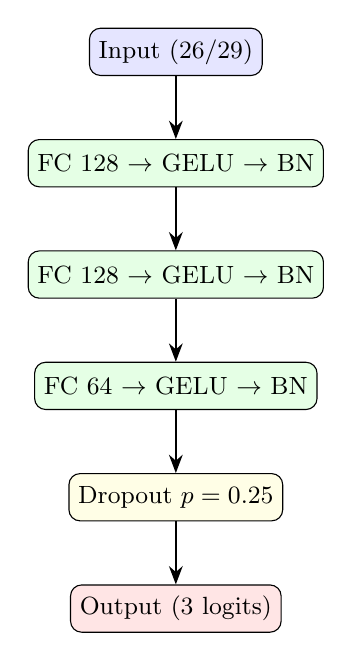
\begin{tikzpicture}[
  neuron/.style={circle, draw, minimum size=0.7cm, inner sep=1pt, font=\tiny},
  layer/.style={rectangle, draw, rounded corners, minimum width=2cm, minimum height=0.6cm, font=\small},
  arrow/.style={-Stealth, thick}
]
  % Input layer
  \node[layer, fill=blue!10] (input) {Input (26/29)};
  % Hidden layers
  \node[layer, fill=green!10, below=0.8cm of input] (h1) {FC 128 $\rightarrow$ GELU $\rightarrow$ BN};
  \node[layer, fill=green!10, below=0.8cm of h1] (h2) {FC 128 $\rightarrow$ GELU $\rightarrow$ BN};
  \node[layer, fill=green!10, below=0.8cm of h2] (h3) {FC 64 $\rightarrow$ GELU $\rightarrow$ BN};
  % Dropout
  \node[layer, fill=yellow!10, below=0.8cm of h3] (drop) {Dropout $p=0.25$};
  % Output
  \node[layer, fill=red!10, below=0.8cm of drop] (output) {Output (3 logits)};
  % Arrows
  \draw[arrow] (input) -- (h1);
  \draw[arrow] (h1) -- (h2);
  \draw[arrow] (h2) -- (h3);
  \draw[arrow] (h3) -- (drop);
  \draw[arrow] (drop) -- (output);
\end{tikzpicture}
\caption{Architecture of the proposed TabularMLP. The network consists of an input layer (26 or 29 neurons), three hidden layers (128, 128, 64) each followed by GELU activation and Batch Normalization, a Dropout layer for regularization, and an output layer with three logits corresponding to the WESAD classes.}
\label{fig:mlp_architecture}
\end{figure}

\subsubsection{Training Strategy}

The training procedure was designed for a small tabular physiological dataset, where two risks are especially relevant: overfitting and class imbalance. Overfitting occurs when the model adapts too closely to the training windows and loses generalization capacity on validation windows. Class imbalance occurs when one affective state has more samples than the others, which can make accuracy misleading because a model may perform well on the majority class while failing on less frequent classes.

Optimization was performed with AdamW\cite{loshchilov2019decoupled}, using an initial learning rate of $2 \times 10^{-3}$ and weight decay of $10^{-3}$. AdamW is an adaptive optimization method that updates each model parameter according to the observed gradients while applying weight decay as a separate regularization term. In practical terms, this discourages excessively large weights and helps reduce overfitting in small datasets. Training was performed in mini-batches of 64 samples, allowing the model to learn from shuffled subsets of the training data rather than recalculating each update from the full dataset at once.

The loss function was class-weighted cross-entropy \cite{goodfellow2016deep}. Cross-entropy is suitable for this task because the model outputs one score for each target class, corresponding to \textit{amusement}, \textit{baseline}, and \textit{stress}. The class weights are computed from the training-label frequencies, assigning a larger penalty to errors in less frequent classes. This prevents the optimization process from being dominated only by the most common affective state. An additional sampling-based rebalancing strategy was also evaluated, in which less frequent classes are sampled more often during training. It was not adopted as the default strategy because combining this sampling policy with class-weighted loss can overcompensate minority classes in small datasets.

Model selection was based on validation macro F1-score\cite{sokolova2009systematic}, not on accuracy. Macro F1 computes the F1-score independently for each class and then averages the three values, giving equal weight to all affective states. This criterion is more appropriate for the WESAD experiments because the objective is not merely to maximize the number of correct predictions, but to maintain balanced performance across \textit{amusement}, \textit{baseline}, and \textit{stress}. The model retained for comparison is therefore the one obtained at the epoch with the highest validation macro F1-score, subject to a minimum improvement threshold of $10^{-4}$.

The training procedure also includes mechanisms to control convergence\cite{goodfellow2016deep}. The learning rate is reduced by a factor of 0.5 when validation macro F1-score stops improving for 15 consecutive epochs, with a minimum learning rate of $10^{-6}$. Early stopping interrupts training when validation macro F1-score does not improve for 50 epochs, avoiding unnecessary optimization after the model has saturated. Finally, gradient clipping limits the gradient norm to 1.0, reducing the risk of unstable parameter updates during backpropagation.

\begin{table}[htbp]
\centering
\caption{Model architecture and training hyperparameters of the baseline MLP and proposed TabularMLP.}
\label{tab:model_and_training}
\footnotesize
\renewcommand{\arraystretch}{1.05}
\resizebox{\textwidth}{!}{%
\begin{tabular}{p{2.0cm} p{3.0cm} p{3.8cm} p{2.2cm} p{3.0cm}}
\toprule
\textbf{Aspect} & \textbf{Baseline MLP} & \textbf{Proposed TabularMLP} & \textbf{Value} & \textbf{Purpose} \\ \midrule
Hidden layers & Two FC layers & Three FC (128, 128, 64) & — & — \\ \midrule
Activation & ReLU & GELU\cite{hendrycks2016gelu} & — & — \\ \midrule
Normalization & Not used & BatchNorm1d\cite{ioffe2015batch} & — & — \\ \midrule
Regularization & Limited & Dropout\cite{srivastava2014dropout} + AdamW weight decay & wd=$10^{-3}$, drop=0.25 & Prevents overfitting in small dataset \\ \midrule
Output & 3 class logits & 3 class logits & — & — \\ \cmidrule{1-5}
Optimizer & — & AdamW\cite{loshchilov2019decoupled} & $2\times10^{-3}$ & Adaptive optimization with decoupled weight regularization \\ \midrule
Batch size & — & 64 & 64 & Samples per optimization step \\ \midrule
Max epochs & — & 300 & 300 & Upper bound on training passes \\ \midrule
LR scheduling & — & Reduce on plateau & factor 0.5, patience 15 & Refines when macro F1 stagnates \\ \midrule
Early stopping & — & Patience 50 & 50 epochs & Stops after no improvement \\ \midrule
Gradient clipping & — & Norm 1.0 & 1.0 & Prevents unstable gradient updates \\ \bottomrule
\end{tabular}%
}
\end{table}


\subsubsection{Augmentation and Class Rebalancing}

The scaled models use online Gaussian noise augmentation \cite{goodfellow2016deep} after standardization. In this setting, a noise value such as $0.03$ has the same meaning for all features because the scaler places them in approximately comparable units.

The no-scaler models cannot safely use the same absolute noise. Without standardization, each feature has its own unit and magnitude; a fixed perturbation can be irrelevant for a large-scale feature and destructive for a small-scale feature. Therefore, the selected no-scaler experiments use online per-feature robust noise. The noise magnitude is proportional to a robust scale estimated from the training split, approximately $\mathrm{IQR}/1.349$, and augmented values are clipped between the 1st and 99th training quantiles. The augmentation probability is $0.5$ and the noise fraction is $0.02$.

This augmentation is online: it does not permanently expand the stored dataset. Instead, batches may receive different controlled perturbations across epochs. Sampling-based class rebalancing was also evaluated as an additional class-imbalance mechanism, but it did not improve the selected no-scaler variant.

Figures~\ref{fig:wesad_f1_curves} and~\ref{fig:wesad_val_loss} show how macro F1-score and validation loss evolved across training epochs for the evaluated configurations.

\begin{figure}[htbp]
\centering
\safeincludegraphics[width=0.92\textwidth]{imagens/wesad_no_scaler/val_f1_macro_curves.png}
\caption{Validation macro F1-score curves for all WESAD training configurations across epochs. The scaled \textit{New full} model reaches the highest local-validation peak (0.9565 at epoch 77), while the selected no-scaler variant favors deployment consistency.}
\label{fig:wesad_f1_curves}
\end{figure}

Figure~\ref{fig:wesad_val_loss} complements this analysis by tracking validation loss throughout training. Validation loss measures how costly the model's predictions are on unseen validation samples; lower values indicate that the predicted probabilities are closer to the correct labels. Across the best-performing scaled configurations, loss decreases during the initial epochs and then stabilizes as learning-rate reduction and early stopping intervene. The \textit{New full} model achieves the lowest validation loss at its best checkpoint ($0.1454$ at epoch 77), whereas the original baseline retains a higher loss ($0.2279$ at epoch 38) despite reaching its F1 peak earlier. The selected no-scaler configuration has a higher validation loss ($0.3526$ at epoch 117), which reflects the cost of removing feature standardization. This result is acceptable for the prototype because the no-scaler model is more consistent with the real data path used by the embedded sensing flow, simulated data flow, and federated learning components.

\begin{figure}[htbp]
\centering
\safeincludegraphics[width=0.92\textwidth]{imagens/wesad_no_scaler/val_loss_curves.png}
\caption{Validation loss curves for all WESAD training configurations. Lower and more stable validation loss at the best epoch indicates better fit to unseen windows; the scaled \textit{New full} model reaches the lowest local-validation loss.}
\label{fig:wesad_val_loss}
\end{figure}

\FloatBarrier

\subsection{Experimental Classification Results}

Eleven training configurations were evaluated to separate model quality, privacy-oriented feature selection, preprocessing reproducibility, and embedded feasibility. These configurations address four experimental questions. The original baseline establishes whether a simple MLP is already sufficient for the extracted features, providing a reproducible reference point. The New full configuration measures the best local validation performance with all features and standardization, serving as the upper local-performance reference. The no-demographics and no-scaler variants quantify the cost of privacy-oriented and deployment-oriented constraints, removing quasi-identifiers and avoiding scaler synchronization across services. The ESP-friendly configurations estimate the feasibility of simplified sensor-side processing using a reduced feature set.

Table~\ref{tab:wesad_results} summarizes the best validation performance achieved by each configuration, ranked by validation macro F1-score. The New full model reached its optimum at epoch 77 out of a maximum of 300, terminating at epoch 127 due to early stopping. The selected no-scaler model peaked later at epoch 117 and stopped at epoch 167. These values indicate that convergence typically required between 77 and 117 epochs across configurations, with the no-scaler variant needing more iterations due to the absence of standardization. Figure~\ref{fig:wesad_core_metrics} compares accuracy, precision, recall, and macro F1 at the best epoch of each experiment.

\begin{table}[htbp]
\centering
\caption{Best validation metrics per training configuration on the WESAD 30-second window dataset.}
\label{tab:wesad_results}
\resizebox{\textwidth}{!}{%
\begin{tabular}{lcccccc}
\toprule
\textbf{Configuration} & \textbf{Features} & \textbf{Best Epoch} & \textbf{Val F1 Macro} & \textbf{Val Accuracy} & \textbf{Val Precision} & \textbf{Val Recall} \\ \midrule
New full (best local) & 29 & 77 & \textbf{0.9565} & 0.9653 & 0.9605 & 0.9531 \\ \midrule
New + weighted sampler & 29 & 156 & 0.9513 & 0.9604 & 0.9472 & 0.9557 \\ \midrule
New without demographics & 26 & 79 & 0.9378 & 0.9455 & 0.9310 & 0.9458 \\ \midrule
New no demo + weighted sampler & 26 & 129 & 0.9265 & 0.9356 & 0.9177 & 0.9374 \\ \midrule
Original baseline MLP & 29 & 38 & 0.9241 & 0.9406 & 0.9406 & 0.9127 \\ \midrule
New no demo no scaler (selected) & 26 & 117 & 0.8307 & 0.8465 & 0.8194 & 0.8546 \\ \midrule
New no demo no scaler + weighted sampler & 26 & 147 & 0.8093 & 0.8218 & 0.7994 & 0.8459 \\ \midrule
ESP-friendly + weighted sampler & 13 & 155 & 0.7693 & 0.7921 & 0.7638 & 0.7991 \\ \midrule
ESP-friendly level 1 + weighted sampler & 13 & 155 & 0.7693 & 0.7921 & 0.7638 & 0.7991 \\ \midrule
ESP-friendly & 13 & 119 & 0.7627 & 0.7921 & 0.7559 & 0.7794 \\ \midrule
ESP-friendly level 1 & 13 & 119 & 0.7627 & 0.7921 & 0.7559 & 0.7794 \\ \bottomrule
\end{tabular}%
}
\end{table}

\begin{figure}[htbp]
\centering
\safeincludegraphics[width=0.95\textwidth]{imagens/wesad_no_scaler/best_core_metrics.png}
\caption{Comparison of core validation metrics at the best epoch selected by macro F1-score for each WESAD training configuration.}
\label{fig:wesad_core_metrics}
\end{figure}

The \textit{New full} configuration achieved the highest local validation macro F1-score, 0.9565 at epoch 77, outperforming the original baseline score of 0.9241 by approximately 3.2 percentage points. Its validation loss \cite{goodfellow2016deep} was also the lowest among the evaluated models (0.1454), and its overfitting gap was small (0.0145, see Figure~\ref{fig:wesad_overfit}). This indicates that the regularized TabularMLP improved local generalization compared with the simpler baseline, whose overfitting gap was 0.0728.

Removing demographic features produced a modest decrease when \texttt{StandardScaler} was still used: the macro F1-score moved from 0.9565 to 0.9378. This supports the privacy-oriented decision to exclude \texttt{age}, \texttt{height}, and \texttt{weight}; most of the discriminative signal remained in the physiological features.

The decisive engineering comparison, however, was not only the highest local F1-score. The model also needed a preprocessing contract that could be reproduced in the embedded and simulated data flow, local training clients, server-side validation, and mobile inference. Under this criterion, the selected integration model was \textit{New no demo no scaler}. It reached 0.8307 macro F1 locally, below the scaled no-demographics model, but it avoids the requirement to broadcast and reproduce scaler statistics across all parts of the system. Weighted sampling did not improve this variant (0.8093), suggesting that class-weighted loss was sufficient for the current dataset.

The ESP-friendly models obtained lower macro F1-scores, between 0.7627 and 0.7693. This result suggests that the removed features, especially EDA decomposition and BVP peak frequency, carry useful classification signal. Nevertheless, these experiments remain important because they quantify the cost of simplifying the feature set for embedded computation.

\begin{figure}[htbp]
\centering
\safeincludegraphics[width=0.88\textwidth]{imagens/wesad_no_scaler/overfit_gap_f1.png}
\caption{Overfitting gap, calculated as training F1 macro minus validation F1 macro, at the best epoch for each configuration. Lower values indicate better generalization; the comparison helps distinguish local validation performance from deployment-oriented model selection.}
\label{fig:wesad_overfit}
\end{figure}

Figure~\ref{fig:wesad_best_epoch} reports the epoch at which each configuration achieved its highest validation macro F1-score. An epoch corresponds to one complete pass through the training set. The \textit{New full} model reaches its optimum at epoch 77 and terminates training at epoch 127 due to early stopping, demonstrating efficient convergence within roughly one quarter of the 300-epoch budget. The selected no-scaler model reaches its best F1 macro at epoch 117 and terminates at epoch 167, showing that removing standardization makes optimization harder but still viable. In contrast, the original baseline peaks as early as epoch 38 but at a substantially lower F1 value than the best scaled model, suggesting rapid memorization of the training set rather than robust learning. These timing differences are relevant for federated deployment: local training nodes at healthcare institutions benefit from models that converge reliably without excessive computational cost per federated round.

\begin{figure}[htbp]
\centering
\safeincludegraphics[width=0.82\textwidth]{imagens/wesad_no_scaler/best_epoch.png}
\caption{Best epoch selected by validation macro F1-score for each training configuration. Earlier peaks with higher F1, such as \textit{New full} at epoch 77, indicate more efficient training; later peaks, such as weighted sampler variants, reflect slower convergence under aggressive class rebalancing.}
\label{fig:wesad_best_epoch}
\end{figure}

Taken together, the experimental figures provide two complementary conclusions. From a purely local validation perspective, the scaled \textit{New full} TabularMLP achieves the best validation macro F1-score (0.9565), the lowest validation loss among the evaluated models (0.1454), and a small overfitting gap (0.0145), while converging in a moderate number of epochs. From a deployment perspective, the selected \textit{New no demo no scaler} model is more appropriate for the federated prototype because it removes demographic attributes and avoids an external scaling dependency that was not consistently reproducible across embedded and simulated data paths, local training clients, server validation, and mobile inference. Thus, the project prioritizes a model with lower local F1 macro (0.8307) but a more reliable end-to-end preprocessing contract.

\FloatBarrier

\subsection{Integration with Federated Learning}

The integration with federated learning was implemented by separating the local data ingestion service from the federated training process. This separation was an important architectural decision because the hospital-side HTTP API should not become responsible for coordinating training rounds, storing model weights, or uploading model files to a central endpoint. Instead, the local API only receives authenticated physiological windows and persists them in the local PostgreSQL database. The federated training responsibility is assigned to a Python service running in the same institutional environment, implemented as a Flower client. On the global side, a Flower server coordinates the rounds, aggregates the received model updates, and publishes the newest global model through a separate Global Model API. The overall organization of this implementation is illustrated in Figure~\ref{fig:federated_integration_architecture}, which provides a visual summary of how the mobile gateway, hospital-side ingestion services, local Flower clients, global Flower server, and model distribution API are connected.

\begin{figure}[htbp]
\centering
\safeincludegraphics[width=0.85\textwidth]{imagens/architeture/federated_integration_architecture.png}
\caption{Implemented federated learning integration architecture, showing the separation between mobile data submission, hospital-side data ingestion, local Flower training, global aggregation, and model redistribution.\protect\footnote{Code Implementation: \protect\url{https://github.com/rodrigomarchiolli/Federated_TOR}}}
\label{fig:federated_integration_architecture}
\end{figure}

The main software contracts in the federated learning integration are distributed across five components. The Local API receives HMAC-authenticated physiological windows, validates requests, and persists accepted records in PostgreSQL. The PostgreSQL database stores accepted sensor windows locally. The Local Flower client reads local database records and global parameters, trains the TabularMLP locally, and returns updated model parameters and metrics. The Global Flower server coordinates federated rounds and aggregates parameters using FedAvg. Finally, the Global Model API publishes the latest ONNX model and metadata for mobile retrieval.

\subsubsection{Local Flower Client Integration at the Local Node}

The local Flower client is deployed alongside the local API and the local PostgreSQL database. Its role is to transform the records accumulated by the API into a federated learning contribution. During each Flower round, the client receives the current global parameters from the server. These parameters are the numerical weights and biases of the neural network, not patient records. The client then reads the available rows from the local sensor table, maps textual labels such as \texttt{amusement}, \texttt{baseline}, and \texttt{stress} to numeric classes, and prepares the 26 physiological input features used by the privacy-oriented TabularMLP configuration. Demographic attributes are intentionally excluded from this federated contract, preserving the same privacy rationale evaluated in the WESAD experiments.

Before local optimization, the client performs preprocessing entirely inside the institutional boundary. Missing feature values are imputed using medians computed from the local training split, invalid labels are discarded, and the local dataset is divided into training and validation partitions when enough samples are available. For the integration path, this preprocessing deliberately avoids \texttt{StandardScaler}, so that the model receives features in the same numerical scale used by the embedded and simulated data paths and the server-side validation routine. The training routine follows the same model family validated experimentally: a multilayer perceptron with Batch Normalization, GELU activations, dropout, AdamW optimization, class-weighted cross-entropy, learning-rate scheduling, gradient clipping, and early stopping based on validation macro F1-score. The client returns only the updated model parameters and training metrics to Flower; the physiological records remain in the hospital database.

The implementation also handles operational edge cases required for a federated deployment. If the database contains no usable samples, or fewer samples than the minimum required for a meaningful local update, the client skips the training step and reports a zero-example result with a controlled status. This behavior prevents an empty hospital node from corrupting the aggregation stage while still allowing the server to continue coordinating other participants. Therefore, this local training service acts as the bridge between the privacy-preserving ingestion pipeline and the federated coordination layer, without expanding the HTTP API beyond its data collection scope.

\subsubsection{Global Flower Server Coordination and Aggregation}

The global Flower server initializes the global TabularMLP model and listens for participating local clients. Communication between the server and clients uses Flower's federated training protocol over gRPC, a remote procedure call mechanism commonly used for communication between distributed services. Its coordination loop follows the standard federated learning pattern: the current global parameters are distributed to selected clients, each client trains locally using its private database, and the server receives the resulting parameter updates. The aggregation strategy is based on FedAvg, which computes a weighted average of client updates according to the number of local examples reported by each participant.

The global strategy was extended with two practical responsibilities. First, it filters ineffective rounds by skipping aggregation when all clients report zero examples, which can occur when no institution has accumulated enough local data. Second, after a successful aggregation, it materializes the global model lifecycle. The aggregated parameters are loaded back into the TabularMLP architecture, saved as a PyTorch checkpoint for traceability, evaluated when a validation dataset is available, exported to ONNX, and published as the latest model artifact. A checkpoint is a saved copy of the model state at a specific training round; it allows later inspection, rollback, or reexport. This lifecycle makes the federated server more than a transient coordinator: it becomes the source of versioned global models that can be audited, rolled back, or redistributed.

\subsubsection{Global Model Distribution to the Mobile Application}

The model redistribution path shown in Figure~\ref{fig:federated_integration_architecture} is intentionally separated from the Flower training protocol. The mobile application does not communicate directly with the Flower server. This distinction is relevant because Flower uses a federated training protocol rather than a public model download API. For inference on the smartphone, the project introduces a Global Model API that exposes the latest exported model and its metadata through conventional HTTP endpoints. The endpoint \texttt{/model/latest} serves the current ONNX file, while \texttt{/model/latest/metadata} returns information such as the federated round, model identifier, file hash, file size, expected input dimension, feature names, output labels, participating clients, and aggregated metrics. The file hash allows the mobile application to verify whether the downloaded model matches the published metadata, and the feature list tells the application the exact order and meaning of the numerical inputs expected by the model.

Publishing the model in ONNX reduces coupling between the mobile application and the internal PyTorch representation used during training. The mobile side can download a stable inference artifact and validate its metadata before using it locally, while the Flower server remains free to store internal checkpoints in PyTorch format. This design closes the federated loop proposed by the architecture: the mobile gateway contributes labeled physiological windows to the local institution, the local Flower client uses those records for local training, the global Flower server aggregates model updates across institutions, and the Global Model API returns the newest global model to the mobile application for local inference.

In the current prototype, the local WESAD experiments validate the quality and trade-offs of the model family that each local Flower client is expected to train, and the implemented Flower components define the operational path for federated rounds and global model publication. The selected integration model is not the highest-scoring local model; it is the no-demographics, no-scaler variant chosen because its preprocessing contract can be reproduced across the complete system. A full multi-institutional benchmark with independent hospital datasets remains a future evaluation step, but the integration already establishes the principal software contracts required for privacy-preserving federated learning: local-only data storage, parameter-based communication, global aggregation, versioned model export, and mobile-oriented model distribution.

\FloatBarrier

\subsection{Limitations of the Current Evaluation}

Five limitations warrant explicit acknowledgment:

\begin{enumerate}[leftmargin=*]
\item \textbf{Window-level split:} the WESAD train/validation split was performed at the window level rather than the subject level, meaning windows from the same participant may appear in both partitions. This may moderately inflate validation metrics relative to true out-of-subject generalization.

\item \textbf{No-scaler performance trade-off:} the selected no-scaler model achieved lower local validation performance than the best scaled model. This was an intentional engineering trade-off: removing \texttt{StandardScaler} reduced local macro F1-score but avoided a preprocessing dependency that was not reliably reproducible across embedded and simulated data paths, local training clients, server validation, and mobile inference.

\item \textbf{Controlled transmission tests:} the mobile-to-Tor transmission path was validated with controlled test payloads. Live integration with continuous ESP32 physiological streams remains an ongoing deployment step.

\item \textbf{No multi-institutional benchmark yet:} although the local Flower client and global Flower server components define the federated execution path, the present evaluation does not yet report a multi-institutional experiment with independent hospital nodes and heterogeneous local distributions.

\item \textbf{Absence of personalization:} the model was trained in an aggregated cross-subject manner without individual calibration or fine-tuning. Since physiological stress thresholds (e.g., EDA, heart rate variability, temperature) vary across individuals, a one-size-fits-all model may not correctly capture the stress/non-stress boundary for each person. Future work should investigate personalization strategies such as per-subject local fine-tuning within the federated client, which is architecturally compatible with the proposed federated framework \cite{ereno2025avaliando}.

\item \textbf{Mobile gateway as single point of failure:} the current architecture routes all physiological data through the mobile application. If the gateway device goes offline or loses network connectivity, data transmission to the local training node is interrupted. Future work should investigate fault-tolerant designs, such as store-and-forward mechanisms on the ESP32 side or multi-gateway redundancy, to mitigate this limitation.

\end{enumerate}

Future work will address subject-level cross-validation, end-to-end latency characterization under Tor routing, and federated evaluation across multiple participating nodes.

\section{Discussion of the Implications Discovered}

The practical results reinforce the central thesis of this research: occupational stress monitoring can be pursued through a layered privacy architecture that combines federated learning with complementary anonymization and authentication mechanisms. Four implications emerge from the implementation.

First, the prototype shows that privacy preservation must begin before data reach the smartphone. The Bluetooth sensing channel was not treated as a neutral transport link; instead, it was constrained by authenticated bonding, persistent ownership, and authorization checks before physiological records or acknowledgement commands could be exchanged.

Second, delegating Tor connectivity to the mobile gateway resolves a fundamental tension between privacy and hardware constraints. Embedded wearables remain responsible for data acquisition, while the smartphone, already present in occupational settings, assumes the role of anonymized communication endpoint. This division of labor is scalable and avoids overburdening resource-limited microcontrollers.

Third, the combination of Tor and HMAC demonstrates that network anonymity and application-layer authentication address distinct threat models and must coexist. Tor alone would allow any anonymous actor to submit data to the hidden service; HMAC alone would authenticate requests but expose the client's network identity. Their joint deployment aligns with the defense-in-depth principle advocated in the federated learning literature reviewed in Section 3.

Fourth, the classification experiments indicate that a regularized tabular MLP achieves strong stress detection performance on window-aggregated physiological features. The scaled privacy-oriented variant, excluding demographic attributes, retained over 98\% of the full model's macro F1-score, while the selected no-scaler variant traded part of this local performance for a preprocessing contract that can be reproduced across embedded and simulated data paths, local training clients, server validation, and mobile inference. This finding supports the feasibility of deploying local models at healthcare institutions without relying on quasi-identifying attributes, while also showing that deployment consistency must be considered alongside validation metrics.

Fifth, the scope clarifications above carry concrete methodological consequences. The stress detection validated in this work corresponds to general physiological arousal under controlled conditions, not to occupational stressors encountered in real work environments. Extrapolating these results to occupational stress monitoring requires caution and further validation in workplace settings. Additionally, the cross-subject aggregated training approach, while practical for initial validation, does not account for the inter-individual variability of physiological stress responses. The federated architecture proposed in this project is, however, inherently compatible with personalization strategies: each client could perform local fine-tuning on subject-specific data, improving the adequacy of stress thresholds for individual users. This direction should be explored in future work.

\section{Conclusion}

This study investigated federated learning as a privacy-preserving approach motivated by occupational stress monitoring, combining a literature review with a practical prototype whose stress classification component was validated for general physiological stress detection (three affective states from the WESAD protocol) rather than for specific occupational stressors. This distinction should be considered when interpreting the findings. The literature review confirmed that federated learning, differential privacy, and secure aggregation techniques are central to protecting sensitive physiological data in distributed health applications. The practical implementation evolved from an ESP32-centric gateway model to a mobile-mediated architecture, in which authenticated Bluetooth bonding restricts local sensor access to the enrolled smartphone, Tor provides topological anonymity, and HMAC-SHA256 ensures authenticated, tamper-evident data submission to local training nodes hosted at healthcare institutions.

Experimental validation on the WESAD dataset demonstrated that the scaled TabularMLP classifier achieves a validation macro F1-score of 0.9565 for three-class affective state classification, outperforming a simpler baseline while maintaining low overfitting. For the federated prototype, the selected no-demographics, no-scaler variant prioritizes reproducible preprocessing across the embedded sensing, simulated data, local training, server validation, and mobile inference paths. Future work will complete live ESP32 stream integration, subject-level cross-validation, Tor latency evaluation, and multi-institutional federated training rounds.

\section*{Use of Artificial Intelligence Tools}
The development of this work involved the use of artificial intelligence tools as assistants in specific stages, as detailed below. All AI-assisted content was reviewed and validated by the authors, who assume full responsibility for the intellectual content of this manuscript.

\begin{itemize}
    \item \textbf{Text writing and revision:} AI-based writing assistants (ChatGPT, Claude) were used for grammar checking, stylistic suggestions, and paragraph organization. No AI tool was used to generate the original research ideas, experimental results, or core scientific contributions.
    \item \textbf{Code implementation:} AI-assisted code generation tools (GitHub Copilot, ChatGPT) were employed to support the implementation of the ESP32 firmware, React Native mobile application, Python training scripts, and Flower federated learning integration. Beyond code generation, the LLMs also aided in researching and interpreting the Tor (onion routing) and HTTP communication protocols, understanding the HMAC-SHA256 signing mechanism for request authenticity and integrity, and creating automated tests for the web system. Additionally, the LLMs assisted with the Bluetooth Low Energy (BLE) communication protocols between the ESP32 and the mobile device, and with native library builds for the mobile application using the Expo framework. All generated code and technical content was reviewed and tested by the authors before integration.
    \item \textbf{Figure and diagram generation:} The system architecture diagram (Figure~\ref{fig:architecture}) was initially drafted by the authors, and generative AI was used to produce a refined version with improved visual design. The mobile application screen designs were created using Google's Stitch (an AI-assisted design tool based on generative AI and LLMs) with Material Design as the visual design system reference.
\end{itemize}

\bibliographystyle{sbc}
\bibliography{sbc-template}

\appendix
\section*{Appendix A: Glossary of Technical Terms}
\label{app:glossary}

\begingroup
\small
\setlength{\tabcolsep}{4pt}
\renewcommand{\arraystretch}{1.08}

\begin{longtable}{p{2.5cm} p{4.7cm} p{6.4cm}}
\caption{Glossary of technical terms used in the prototype description.}
\label{tab:technical_terms_results} \\

\toprule
\textbf{Term} & \textbf{Meaning} & \textbf{Role in this project} \\ \midrule
\endfirsthead

\caption[]{Glossary of technical terms used in the prototype description. (Continued)} \\

\toprule
\textbf{Term} & \textbf{Meaning} & \textbf{Role in this project} \\ \midrule
\endhead

\bottomrule
\endfoot

IoMT & \textit{Internet of Medical Things}; connected medical or health-related sensing devices. & Sensing layer composed of wearable physiological sensors connected to the ESP32. \\ \midrule

ESP32 & Low-cost microcontroller with wireless communication capabilities. & Local sensing unit controller that receives pre-stored signals from wearable sensors and sends them to the mobile application through authenticated Bluetooth Low Energy bonding. \\ \midrule

Bluetooth Low Energy (BLE) bonding & Persistent authenticated pairing between a peripheral device and a central device. & Restricts local sensor access to the smartphone that completed authenticated enrollment with the sensing unit. \\ \midrule

BVP, EDA, TEMP, Resp & Physiological signals related to blood volume pulse, electrodermal activity, skin temperature, and respiration. & Basis for stress-related feature extraction and classification. \\ \midrule

Mobile Gateway & Smartphone application that mediates communication between the sensing layer and the institutional node. & Receives ESP32 data, stores credentials, signs requests, routes traffic through Tor, and supports user interaction. \\ \midrule

Tor & An anonymity network based on onion routing. & Hides the network origin of requests sent by the mobile application to the hospital-side hidden service. \\ \midrule

HMAC-SHA256 & Cryptographic message authentication mechanism based on a shared secret and SHA-256 hashing. & Verifies request authenticity and integrity before physiological data are accepted by the local API. \\ \midrule

PostgreSQL & Relational database management system. & Stores authenticated physiological windows locally inside the institutional environment. \\ \midrule

Flower & Federated learning framework for coordinating distributed model training. & Implements communication between local training clients and the global federated server. \\ \midrule

FedAvg & \textit{Federated Averaging}; aggregation rule for combining model updates from multiple clients. & Aggregates local model parameters into a global model without centralizing raw physiological data. \\ \midrule

ONNX & Open Neural Network Exchange; interoperable format for machine learning models. & Exports the updated global model for mobile-oriented inference and redistribution. \\

\end{longtable}

\endgroup

\end{document}
